\section{Processi di supporto}

\subsection{Documentazione}

\subsubsection{Scopo}
Lo scopo di questo processo è quello di redigere e mantenere la documentazione durante tutto il ciclo di vita del software
I documenti formali che verranno presentati saranno suddivisi in due categorie:

\begin{itemize}
\item[•] \textbf{Interni}:
	\begin{list}{$\circ$}{}
		\item \textbf{Norme di progetto}: lo scopo del documento è di stabilire convenzioni e norme che il team SWEight dovrà seguire durante tutto il progetto;	
	    \item \textbf{Studio di fattibilità}: il documento presenterà il processo che ha portato il team alla scelta del capitolato, riportando le motivazioni di preferenza o rifiuto di ogni capitolato.
    \end{list} 
\item[•] \textbf{Esterni}:
	\begin{list}{$\circ$}{}
		\item \textbf{Piano di progetto}: documento per l’analisi e la pianificazione della gestione delle risorse di tempo e umane;
		\item \textbf{Piano di qualifica}: documento che descrive standard e obiettivi che il gruppo deve raggiungere per garantire la qualità di processo e prodotto;
		\item \textbf{Glossario}: documento che raccoglie tutte le definizioni dei termini poco frequenti utilizzati in tutti i documenti del progetto;
		\item \textbf{Analisi dei requisiti}: documento che contiene l’analisi dei casi d’uso del prodotto e i diagrammi di interazioni previste con l’utente.
	\end{list}
\end{itemize}

\subsubsection{Template}
Per semplificare e standardizzare la stesura dei documenti previsti è stato creato un template \LaTeX{} contenente tutte le impostazioni per la struttura grafica e lo stile di formattazione. Ogni membro del team deve obbligatoriamente utilizzare questo template.
\subsubsection{Versioni}
Per ogni documento deve essere specificata obbligatoriamente la versione nella seguente forma: 
\begin{center}
\textbf{X.Y.Z}
\end{center}
Dove X, Y, e Z sono interi non negativi. X viene incrementata ad ogni revisione, Y viene incrementata ogni qualvolta venga inserito un nuovo capitolo, infine Z determina le modifiche al documento. Ogni elemento deve incrementare indipendentemente. Per esempio: 1.9.0 $\rightarrow$ 1.10.0 $\rightarrow$ 1.11.0 .

%\begin{itemize}
%\item[•]La versione Major zero (0.y.z) è per lo sviluppo iniziale;
%\item[•]X: la versione Major (X.y.z | X > 0) identifica la versione di rilascio. Deve essere incrementata se è stata introdotta qualsiasi modifica non retrocompatibile. Le versioni Patch e Minor devono essere reimpostate a 0 quando la versione Major è incrementata;
%\item[•]Y: la versione Minor (x.Y.z | x > 0) deve essere incrementata se è stata introdotta una nuova funzionalità. La versione Patch deve essere reimpostata a 0 quando la versione Minor è incrementata;
%\item[•] Z: la versione Patch (x.y.Z | x > 0) deve essere incrementata solo se sono state introdotte correzioni retrocompatibili di bug. Una correzione di un bug è definita come una modifica interna che corregge un comportamento errato.
%\end{itemize}
%Una volta che un pacchetto versionato è stato rilasciato, i contenuti di quella versione non devono essere modificati. Qualsiasi modifica deve essere rilasciata come una nuova versione.

\subsubsection{Struttura}
Ogni documento deve essere realizzato a partire dal template descritto precedentemente, la cui struttura non deve essere modificata, ad eccezione dei verbali e della lettera di presentazione, dovrà essere composta da:
\begin{itemize}
\item[•] \textbf{Frontespizio}: questa sezione si trova nella prima pagina di ogni documento e deve contenere:
     \begin{list}{$\circ$}{}
		\item \textbf{Logo}: logo del gruppo;
		\item \textbf{Titolo}: titolo del documento;
		\item \textbf{Nome del gruppo};
		\item \textbf{Nome del progetto};
		\item \textbf{E-mail}: indirizzo di posta elettronica in comune per le comunicazioni interne ed esterne;
		\item \textbf{Versione}: versione del documento;
		\item \textbf{Owner}: responsabile del documento;
		\item \textbf{Redattori}: redattori del documento;
		\item \textbf{Verificatori}: verificatori del documento;
		\item \textbf{Uso}: interno o esterno;
		\item \textbf{Distribuzione}: destinatari del documento;
		\item \textbf{Descrizione}: breve descrizione del documento.		
	\end{list}
\item[•] \textbf{Registro delle modifiche}: questo deve essere riportato nella seconda pagina sotto forma di tabella, contenente: versione del documento, data si salvataggio, descrizione della nuova versione, nominativo e ruolo;
\item[•] \textbf{Indice}: contiene il nome di tutti i capitoli, sezioni e sottosezioni seguiti dal numero della pagina iniziale. Nel caso in cui il documento contenga immagini e/o tabelle devono essere presenti anche i relativi indici;
\item[•] \textbf{Indice delle immagini};
\item[•] \textbf{Indice delle tabelle};
\item[•] \textbf{Introduzione}: contiene lo scopo del documento, una breve descrizione ed i vari riferimenti normativi e informativi utili al lettore;
\item[•] \textbf{Contenuto del documento}.
\end{itemize}

% Andrebbe messo un altro sub 
% https://tex.stackexchange.com/questions/60209/how-to-add-an-extra-level-of-sections-with-headings-below-subsubsection

\paragraph{Formattazione delle pagine}\mbox{}\\
Ogni pagina, escluso il frontespizio ed indice, devono contenere:
\begin{itemize}
	\item[•] \textbf{Intestazione}:
	\begin{list}{$\circ$}{}
		\item Logo del gruppo (a sinistra);
		\item Numero del capitolo corrente seguito dal nome (a destra).
	\end{list}
	\item[•] \textbf{Piè di pagina}:
	\begin{list}{$\circ$}{}
	\item Nome e versione del documento (sinistra);
	\item Numero pagina, in formato “N di M” dove N è la pagina corrente ed M è il numero di pagine totali.
	\end{list} 
\end{itemize}

\subsubsection{Norme Tipografiche}
\begin{itemize}
\item[•] \textbf{Maiuscolo}: l'uso del maiuscolo è obbligatorio nei seguenti casi:
	\begin{list}{$\circ$}{}
	\item All'inizio di ogni elemento di un elenco puntato;
	\item Nella scrittura degli acronimi;
	\item Dopo il punto, punto di domanda, punto esclamativo;
	\item Per i ruoli di progetto, i nomi dei documenti, le fasi di progetto, revisioni di progetto oltre a dove previsto dalla lingua italiana;
	\item Per i ruoli di progetto, i nomi dei documenti, le fasi di progetto, revisioni di progetto oltre a dove previsto dalla lingua italiana. 
	\end{list}
\item[•] \textbf{Grassetto}: il grassetto può essere utilizzato solo per evidenziale l’oggetto trattato di un elenco puntato e per le parole chiave;
\item[•] \textbf{Collegamenti}: tutti i collegamenti devono essere di colore rosso;
\item[•] \textbf{Riferimenti a sezioni}: i riferimenti interni al documento devono riportare il numero della sezione, preceduto dal simbolo di paragrafo (esempio §2.1.3);
\item[•] \textbf{Corsivo}: il corsivo deve essere utilizzato nei seguenti casi:
\begin{list}{$\circ$}{}
	\item \textbf{Ruoli}: in ogni nome di ruolo;
	\item \textbf{Documenti}: in ogni nome di documento;
	\item \textbf{Citazioni}: in ogni citazione.
\end{list}

\item[•] \textbf{Codice}: i frammenti di codice devono essere racchiusi in un riquadro di colore nero;
\item[•] \textbf{Glossario}: per contrassegnare che una parola che è presente nel glossario è necessario aggiungere una G maiuscola al pedice della parola (ad esempio: {termine}\ped{G});
\item[•] \textbf{Elenchi puntati}:
\begin{list}{$\circ$}{}
	\item Ogni elemento dell'elenco deve terminare con il punto e virgola, ad eccezione dell'ultimo elemento che deve terminare con il punto;
	\item Gli elementi di primo livello devono avere come stile un pallino pieno nero, quelli di secondo livello un pallino nero vuoto, ad eccezione degli elenchi numerati che devono essere usati solo se è necessario descrivere una sequenza;
	\item Gli elementi di livello successivo al secondo devono alternare lo stile del primo e del secondo livello.
\end{list}
\item[•] \textbf{Citazioni}: ogni citazione deve essere accompagnata dal riferimento bibliografico.
\end{itemize}

%va messo un altro sub 

\paragraph{Formati}\mbox{}\\
Date: ogni data deve seguire lo standard internazionale per date e orari ISO 8601:2004:
\begin{center}
AAAA-MM-GG
\end{center}
dove: 
\begin{itemize}
\item[•] AAAA: rappresenta il formato dell’anno scritto con quattro cifre;
\item[•] MM: rappresenta il formato del mese scritto con due cifre;
\item[•] GG: rappresenta il formato del giorno scritto con due cifre.
\end{itemize}

\subsubsection{Componenti grafiche}
%va messo un altro sub 

\paragraph{Tabelle}\mbox{}\\
Tutte le tabelle devono avere un indice univoco che la identifichi all’interno del documento ed una breve descrizione posizionata sotto di essa. Le intestazioni delle tabelle devono essere in grassetto.

%va messo un altro sub 
\paragraph{Immagini}\mbox{}\\
Tutte le immagini inserite nei vari documenti devono avere un eguale e sufficiente margine orizzontale e verticale in modo da non ridurre la leggibilità del testo. Ogni immagine deve anch’essa avere un indice univoco che la contraddistingua nell’intero documento.

%va messo un altro sub 
\paragraph{Diagrammi UML}\mbox{}\\
Il software che deve essere utilizzato per la creazione dei diagrammi UML è Astah versione 8.0.0, gli analisti devono utilizzare la documentazione del software per il suo studio e utilizzo.
Ogni diagramma di caso d’uso è identificato in alto a sinistra dal suo codice identificativo e dal nome.

\subparagraph{Esportare immagini in Astah}
I diagrammi dovranno essere esportati come immagini secondo le specifiche sotto riportate. Per esportare i diagrammi in Astah, dopo aver completato il diagramma, selezionare: $Tools \rightarrow Export\ image \rightarrow Current\ Diagram \rightarrow PNG$.
L'immagine rappresentante l'UML deve avere le seguenti caratteristiche:
\begin{itemize}
\item Nome file: UC\texttt{Codice Identificativo}, privo di "."\\
Ad esempio: UC4.2.png $\rightarrow$ UC42.png;
\item Formato file immagine \texttt{.png};
\item Massima larghezza 17cm;
\item Didascalia figura con codice caso d'uso;
\item Il file deve essere salvato all'interno del folder img, destinato alle immagini.
\end{itemize}
Inoltre, anche il file con estensione asta deve essere salvato nella cartella predisposta al fine di permetterne modifiche successivamente. 
Per la realizzazione dell'analisi dei requisiti la cartella destinata al salvataggio dei digrammi modificabili è: "Casi d'uso", reperibile all'interno del {branch}\ped{G} Analisi dei Requisiti. Il nome del diagramma deve essere il medesimo dell'immagine esportata.

\subsubsection{Strumenti di supporto}
%va messo un altro sub 
\paragraph{Stesura dei documenti}\mbox{}\\
L'intera documentazione deve essere prodotta utilizzando il {linguaggio di markup}\ped{G} \LaTeX{}, scelto dal team per i seguenti motivi:
\begin{itemize}
\item[•] Gestisce elegantemente e con facilità gli indici, i pedici, i riferimenti ed il glossario;
\item[•] È un linguaggio che supporta il {versionamento}\ped{G};
\item[•] Permette la stesura del documento suddividendolo in parti che rappresentano le varie sezioni, facilitando così la stesura del documento.
\end{itemize}
Per installare \LaTeX{} è necessario installare il compilatore pdflatex, integrato in un software come TexLive reperibile all'indirizzo \url{https://www.tug.org/texlive/}. Quest'ultimo è {cross platform}\ped{G}, {open source}\ped{G} e gratuito. Si consiglia l'installazione del pacchetto completo per evitare di installare pacchetti successivamente.
Per la stesura del documento è consigliato l'utilizzo di Textmaker, le principali caratteristiche sono:
\begin{itemize}
	\item[•] Compilatore e visualizzatore {PDF}\ped{G} per il documento prodotto;
	\item[•] Evidenziazione della sintassi;
	\item[•] Completamento automatico.
\end{itemize}  
Il software è reperibile all'indirizzo \url{http://www.xm1math.net/texmaker/}, è {cross platform}\ped{G} ed è gratuito.


%va messo un altro sub 
\paragraph{Controllo ortografico}\mbox{}\\
Al termine della stesura dei documenti, prima di alla fase di verifica del documento, l’owner deve effettuare un test sulla piattaforma alla pagina: \url{ http://www.corrige.it}, quest’ultima restituirà un’eventuale lista di errori ortografici, errori di sintassi e l’indice Gulpeas.

\subsubsection{Ciclo di vita}
Per gestire il ciclo di vita dei documenti, deve essere utilizzato il servizio di issues offerto da GitHub.
\begin{enumerate}
\item Per iniziare la stesura di un documento l'owner deve assegnarsi una issues (To do);
\item Quando inizia la stesura del documento (In progress):
	\begin{enumerate}
		\item Sposta la issue nella sezione “in progress”;
		\item Crea un branch per lavorare sulla issue.
	\end{enumerate}
\item Finita l'attività di scrittura crea un pull request con (Needs review):
	\begin{enumerate}
		\item Sé stesso come assigneer;
		\item I verificatori come reviewers;
		\item I campi project e milestone vuoti.
	\end{enumerate} 
\item I verificatori controllano il documento e possono:
	\begin{enumerate}
	 	\item Accettarlo (Reviewer approved);
	 	\item Non accettarlo (In progress).
	\end{enumerate}
\item Se non accettato, l’owner deve apportare le modifiche descritte dal verificatore;
\item Se accettato, sarà compito del responsabile di progetto di effettuare il merge e chiudere la issues (Done).
\end{enumerate}
\begin{figure}[H]
\centering
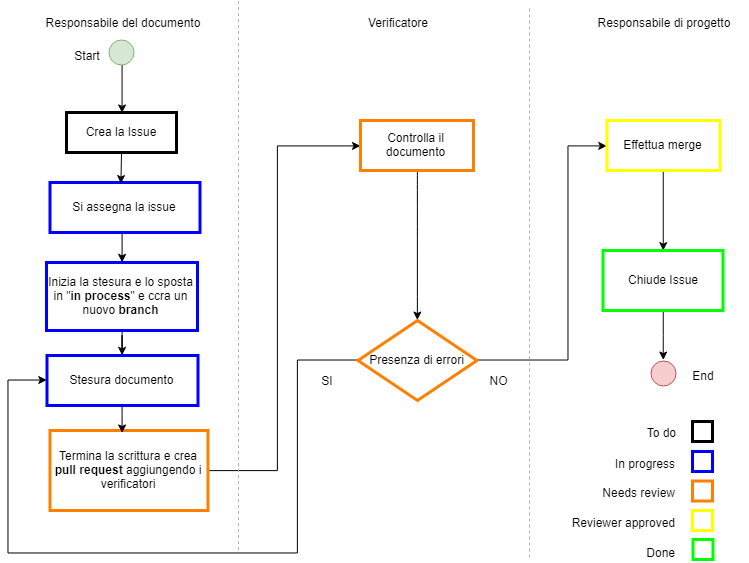
\includegraphics[width=17cm]{img/document_lc.PNG}
\caption{Ciclo di vita di un documento}
\label{fig:document_lifecycle}
\end{figure}

\subsection{Verifica}

\subsubsection{Scopo}

La verifica dei processi, documenti e prodotti è un'attività da eseguire continuamente durante lo sviluppo del progetto. Di conseguenza, servono modalità operative chiare e dettagliate per i Verificatori, in modo da uniformare le attività di verifica svolte ed ottenere il miglior risultato possibile. 

La corretta implementazione del processo deve:
\begin{itemize}
\item[•] Fornire le procedure di verifica necessarie; 
\item[•] Individuare i criteri per la verifica; 
\item[•] Individuare eventuali difetti perché possano essere corretti.
\end{itemize}

\subsubsection{Analisi}

%va aggiunto un sub 
\paragraph{Analisi statica}\mbox{}\\
\begin{itemize}
\item[•] \textbf{Walkthrough}: lettura completa del codice sorgente da analizzare. Va utilizzata unicamente durante le prime fasi del progetto in quanto risulta onerosa e non efficiente, questa tecnica di analisi prevede una lettura critica del codice o del documento prodotto. Gli Analisti che la utilizzano devono stilare una lista di controllo con gli errori rilevati più frequentemente;
\item[•] \textbf{Inspection}: lettura mirata del codice sorgente da analizzare. Questa tecnica di analisi presuppone l’esperienza da parte del verificatore nell’individuare gli errori e le anomalie più frequenti in modo tale da creare una lista di controllo per poter localizzare eventuali punti critici in cui cercare errori. Dopo ogni analisi la lista di controllo deve essere incrementata con eventuali nuovi errori rilevati.
\end{itemize}

%va aggiunto un sub 
\paragraph{Analisi dinamica}\mbox{}\\
Si applica solo alle componenti software e consiste nella verifica e validazione attraverso i test. Per garantire la correttezza è necessario che i test siano ripetibili, dato lo stesso input il test deve produrre sempre lo stesso output.  

Solo i test con queste caratteristiche riescono a verificare la correttezza del prodotto 

Per ogni test deve quindi essere definito: 
\begin{itemize}
\item[•] Ambiente: sistema hardware e software in cui viene eseguito il test; 
\item[•]Stato iniziale: stato iniziale da cui si parte ad eseguire il test; 
\item[•] Input: input inserito;
\item[•] Input: input inserito.
\end{itemize}

\subsubsection{Test}

%va aggiunto un sub 
\paragraph{Test di unità}\mbox{}\\
Il test di unità verifica che ogni singola unità funzioni correttamente, le unità sono specificate nella progettazione di dettaglio.  

In particolare, si verifica che i requisiti per quella determinata unità siano soddisfatti.
\begin{itemize}
\item[•] \textbf{Test strutturale (white-box)}: verifica la logica interna del codice dell’unità cercando la massima copertura. Ogni singola prova deve attivare un singolo cammino di esecuzione all’interno dell’unità. L’insieme di dati di ingresso che ottiene quell’effetto costituisce un caso di prova;
\item[•] \textbf{•} fa riferimento alla specifica dell’unità utilizza dati di ingresso capaci di provocare l’esito atteso. Ciascun insieme di dati di ingresso che produca un dato comportamento funzionale costituisce un singolo caso di prova.
\end{itemize}

%va aggiunto un sub 
\paragraph{Test di Integrazione}\mbox{}\\
Si applica alle componenti specificate nella progettazione architetturale, rappresenta l’estensione logica del test di unità. Consiste nella combinazione di due unità già sottoposte a test in un solo componente e nel test dell’interfaccia presente tra le due. Il test di integrazione consente di individuare i problemi che si verificano quando due unità si combinano. Per effettuare tali test si farà uso di classi appositamente create per simulare e verificare l’interazione.
Strategie di integrazione:
\begin{itemize}
\item[•] \textbf{Assemblare parti in modo incrementale}:
	\begin{list}{$\circ$}{}
		\item Si sviluppano e si integrano prima le parti con minore dipendenza funzionale e maggiore utilità;
		\item Poi si risale l’albero delle dipendenze;
		\item Questa strategia riduce il numero di stub necessari al test ma ritarda la disponibilità di funzionalità di alto livello.
	\end{list}
\item[•] \textbf{Top-down}:
	\begin{list}{$\circ$}{}
	\item Si sviluppano prima le parti più esterne, quelle poste sulle foglie dell’albero delle dipendenze e poi si scende;
	\item Questa strategia comporta l’uso di molti stub ma integra a partire dalle funzionalità di più alto livello.
	\end{list}
\item[•] \textbf{Assemblare produttori prima dei consumatori};
\item[•] \textbf{Assemblare in modo che ogni passo di integrazione sia reversibile}.
\end{itemize}

%va aggiunto un sub 
\paragraph{Test di sistema}\mbox{}\\
Il test di sistema consiste nella validazione del sistema ed è un test di tipo funzionale. Viene eseguito quando si ritiene che il prodotto sia giunto ad una versione definitiva, verificando la completa copertura dei requisiti software. 

%va aggiunto un sub 
\paragraph{Test di regressione}\mbox{}\\
Il test di regressione va eseguito ogni volta che viene modificata un'implementazione in un programma. È possibile eseguire nuovamente i test esistenti sul codice modificato, integrando solo le parti che abbiano precedentemente superato il test di unità, per stabilire se le modifiche apportate hanno alterato elementi precedentemente funzionanti. Se necessario è anche possibile scrivere nuovi test. 
\newline
I contenuti del test di regressione vanno decisi nel momento in cui si approvano modifiche al SW

%va aggiunto un sub 
\paragraph{Test di accettazione (collaudo)}\mbox{}\\
Il test di accettazione consiste nel collaudo del sistema eseguito dal committente. Se l'esito è positivo si può procedere al rilascio ufficiale del prodotto.

\subsubsection{Verifica dei documenti}
Ogni volte che un documento viene modificato, per essere approvato dal Responsabile di progetto, deve essere verificato da un Verificatore. 
\newline
Per essere certi che il documento sia conforme alle norme di progetto e agli altri documenti presentate, il Verificatore deve:
\begin{itemize}
\item[•] Verificare il contenuto: controllare che tutto il contenuto del documento sia inserito nella giusta sezione ed adeguatamente impaginato;
\item[•] Verificare il glossario: controllare che tutte le parole da inserire nel glossario siano state inserite e che tutte le parole inserite nel glossario, siano state targate con il pedice “G”;
\item[•] Verifica tipografica: controllare con il controllo ortografico dell’editor utilizzato eventuali errori e correggerli;
\item[•] Segnalare gli errori: una volta completata la verifica, deve segnalare tutti gli errori trovati e comunicarli al redattore.
\end{itemize}
\paragraph{Regole a garanzia dell'assenza di conflitto di interessi}\mbox{}\\
I redattori dei documenti non possono anche esserne i verificatori. Pertanto è necessario che nessuno dei componenti del gruppo sia messo in condizione di verificare la parte da lui redatta, e quindi affinché ciò non avvenga il gruppo si adopererà attuando una rotazione periodica dei ruoli, o in caso questa non sia possibile, semplicemente assicurarsi che nessun membro verifichi le sezioni dei documenti assegnatoli.
\subsubsection{Verifica dei diagrammi}
I diagrammi devono essere verificati manualmente dal Verificatore che deve controllare che aderiscano correttamente allo standard 2.0. In particolare deve controllare che i diagrammi di flusso siano rappresentati in maniera corretta e che i diagrammi utilizzino correttamente le inclusioni e le estensioni.

\section{Progressi organizzativi}

\subsection{Obiettivo}
Gli obiettivi del processo di gestione sono:
\begin{itemize}
\item[•] Raggiungere l’efficienza e l’efficacia seguendo un approccio sistematico dei processi software al fine di raggiungere gli obiettivi di progetto rispettando le scadenze;
\item[•] Introdurre nuovi processi o migliorare quelli già esistenti.
\end{itemize}

\subsubsection{Incontri}

%va aggiunto un sub 
\paragraph{Interni}\mbox{}\\
Una riunione dell'intero team è richiesta in caso di necessità del Responsabile di progetto. Nel momento in cui un membro del gruppo abbia la necessità di incontrarsi con il team, deve inviare una richiesta al Responsabile di progetto che la valuta e organizza un eventuale incontro. Questi sono fissati solo per discutere di argomenti attinenti al progetto.

%va aggiunto un sub 
\paragraph{Esterni}\mbox{}\\
Il Responsabile di progetto è l'unico a poter fissare gli incontri con il proponente o i committenti e successivamente informare i componenti del team. Non è necessaria la presenza dell’intero gruppo di lavoro durante gli incontri con gli esterni. Il numero di partecipanti sarà quindi limitato a 2 rappresentanti del team di sviluppo.  
\newline
Il Responsabile di progetto deve essere sempre presente agli incontri con gli esterni mentre il secondo partecipante del team è scelto in base all’ordine del giorno. 
\newline
Ogni riunione comprende la stesura di un verbale ufficiale contenente le seguenti informazioni:
\begin{itemize}
\item[•] Data e ora;
\item[•] Luogo;
\item[•] Partecipanti esterni;
\item[•] Partecipanti interni;
\item[•] Ordine del giorno;
\item[•] Domande e risposte.
\end{itemize}

\subsubsection{Comunicazione}

%va aggiunto un sub 
\paragraph{Interna}\mbox{}\\

Per le comunicazioni interne al gruppo è stato adottato {Slack}\ped{G}, un'applicazione di messaggistica multipiattaforma con funzionalità specifiche per gruppi di lavoro.  
\newline
Su Slack si possono integrare {Bot}\ped{G}, creare canali tematici per rendere più efficiente lo scambio e il reperimento delle informazioni, fare ricerche di messaggi vecchi e condividere file di grosse dimensioni.   
\newline
In Slack, sono stati creati dei canali per dividere le comunicazioni con temi comuni:
\begin{itemize}
\item[•] Analisti;
\item[•] Colletta;
\item[•] Norme di progetto;
\item[•] Random;
\item[•] Verifica;
\item[•] Link.
\end{itemize}

%va aggiunto un sub 
\paragraph{Esterna}\mbox{}\\
Per le comunicazioni esterne è stata creata una casella di posta elettronica \href{SWEight@gmail.com}.
\newline 
Tale indirizzo deve essere l'unico canale di comunicazione esistente tra il gruppo di lavoro e l'esterno. 
\newline
Come descritto nel capitolato d'appalto: 
\begin{itemize}
\item[•] La proponente può essere contattata in qualsiasi momento, solo dal responsabile di progetto, attraverso l'indirizzo e-mail \href{tech@mivoq.it} , al quale risponde il reparto tecnologico dell'azienda;
\item[•] Le e-mail devono contenere in oggetto la sigla “UNIPD-SWE" e dovranno essere indirizzate all'attenzione di Giulio Paci, che sarà il referente principale;
\item[•] Ogni e-mail ricevuta su questo indirizzo viene inoltrata automaticamente alla casella personale di ciascun membro, tramite l'utilizzo di filtri di Gmail;
\item[•] In alternativa per una comunicazione ritenute indifferibili è possibile telefonare al numero 0490998335.
\end{itemize}

\subsection{Gestione delle responsabilità e ruoli}

\subsubsection{Introduzione}
I ruoli di progetto rappresentano le figure professionali che lavorano al progetto. Ogni membro del gruppo, in un dato momento, dovrà ricoprire un determinato ruolo.  
\newline
La rotazione è opzionale e si terrà conto delle preferenze personali di ognuno. Ogni membro deve rispettare il proprio ruolo e svolgere le attività assegnategli, secondo quanto stabilito nel Piano di Progetto v 1.0.0. Si avrà l'accortezza di evitare situazioni di conflitto di interesse come, ad esempio, essere verificatori di documenti prodotti da sè stessi, compromettendone cosi la qualità.

\subsubsection{Responsabile di progetto}
Il Responsabile di Progetto, o Project Manager, è una figura necessaria alla gestione dell’intero progetto. Egli raccoglie su di sé le responsabilità decisionali di scelta e approvazione e costituisce il centro di coordinamento per l'intero progetto; in particolare, rappresenta il gruppo di lavoro nei confronti dei Committenti e della Proponente. 
\newline
In particolare, ha l’incarico di:
\begin{itemize}
\item[•] Organizzare incontri interni ed esterni;
\item[•] Pianificare le attività svolte dal gruppo;
\item[•] Individuare per ciascun compito un membro del gruppo per svolgerlo;
\item[•] Analizzare, monitorare e gestire i rischi.
\end{itemize}

\subsubsection{Amministratore di progetto}
L’Amministratore di Progetto è la figura professionale che si deve gestire l’ambiente di lavoro, al fine di aumentare l’efficienza e portare qualità. 
\newline
Ha l'incarico di:
\begin{itemize}
\item[•] Ricercare nuovi strumenti che migliorino l’efficienza;
\item[•] Gestire la documentazione di progetto;
\item[•] Occuparsi del controllo di versione del prodotto;
\item[•] Occuparsi della configurazione del prodotto.
\end{itemize}

\subsubsection{Analista}
L'Analista è la figura che svolge le attività di analisi al fine di comprendere appieno il dominio del problema.  
\newline
Ha l’incarico di:
\begin{itemize}
\item[•] Analizzare i requisiti del prodotto;
\item[•] Analizzare i requisiti di dominio;
\item[•] Redigere il documento Studio di Fattibilità;
\item[•] Redigere il documento Analisi dei Requisiti.
\end{itemize}

\subsubsection{Progettista}
Il Progettista è il responsabile delle scelte architetturali del progetto e ne influenza gli aspetti tecnici e tecnologici.  
\newline
Partendo dalle attività dell'Analista, il Progettista ha il compito di trovare una possibile soluzione per i problemi e i requisiti precedentemente individuati. 
\newline
Ha l’incarico di:
\begin{itemize}
\item[•] Comprendere a fondo i requisiti nel documento Analisi dei Requisiti;
\item[•] Comprendere a fondo i requisiti nel documento Analisi dei Requisiti;
\item[•] Redigere la documentazione tecnica per il prodotto software;
\item[•] Redigere il documento Manuale Sviluppatore.
\end{itemize}

\subsubsection{Programmatore}
Il Programmatore è la figura che provvederà alla codifica della soluzione, studiata e spiegata dal Progettista.  
\newline
Ha l’incarico di:
\begin{itemize}
\item[•] Scrivere il codice del prodotto software che rispetti le decisioni del Progettista;
\item[•] Redigere il documento Manuale Utente.
\end{itemize}

\subsubsection{Verificatore}
Il Verificatore è una figura presente per l'intero ciclo di vita del software e controlla che le attività svolte siano conformi alle attese e alle norme prestabilite.  
\newline
Ha l’incarico di:
\begin{itemize}
\item[•] Verificare che ciascuna attività svolta sia conforme alle norme stabilite nel progetto;
\item[•] Controllare che, per ogni stadio del ciclo di vita del prodotto, questo sia conforme al Piano di Qualifica.
\end{itemize}

\subsection{Pianificazione}
Il Responsabile decide le scadenze tenendo conto degli impegni lavorativi e scolastici di ogni membro. Stima i costi e le risorse necessarie, pianifica le attività e le assegna alle persone. 
\newline
Il responsabile di progetto deve definire il piano di progetto, in cui descrive attività e compiti utili/necessari all’ esecuzione di processo.  
\newline
Il piano deve:
\begin{itemize}
\item[•] Fissare un tempo di completamento dei compiti;
\item[•] Dare una stima del tempo richiesto dei compiti;
\item[•] Adeguare le risorse necessarie per eseguire i compiti;
\item[•] Allocare i compiti;
\item[•] Assegnare le responsabilità; 
\item[•] Analizzare i rischi;
\item[•] Definire delle metriche per il controllo della qualità;
\item[•] Associare dei costi al processo di esecuzione;
\item[•] Fornire un’infrastruttura.
\end{itemize}

\subsection{Monitoraggio del piano}
Il Responsabile di Progetto supervisiona l'esecuzione del progetto fornendo report interni sulla progressione del processo. 
\newline
Egli deve investigare, analizzare e risolvere i problemi scoperti durante l'esecuzione ed eventualmente può rivedere la pianificazione temporale per far fronte a tali problemi e a cambi di strategia.
\begin{itemize}
\item[•] I report redatti, in conclusione di ogni periodo, confluiranno nel Piano di Qualifica;
\item[•] Al termine del periodo di riferimento, il Responsabile di Progetto deve confrontare i risultati ottenuti con gli obiettivi prefissati e valutare strumenti, attività e processi impiegati per il completamento dei processi;
\item[•] La valutazione finale e il tracciamento di strumenti e tecnologie dovranno confluire nel Piano di Qualifica, eventuali rischi e piani di contingenza utilizzati dovranno essere riportati nel Piano di Progetto.
\end{itemize}

\subsection{Gestione dell'infrastruttura}




\subsubsection{Introduzione}
Inizializzare, implementare e gestire processi software, richiede l’istanziazione di un’infrastruttura ad hoc per l'intero progetto. In questa sezione verranno verrà normato e descritto l’ambiente di lavoro e gli strumenti o software utilizzati.

\subsubsection{Versionamento}

%va messo un altro sub 
\paragraph{Introduzione}\mbox{}\\
Git, il più usato e conosciuto {software di controllo di versione}\ped{G} {open source}\ped{G}, è stato scelto per il controllo di versione, GitHub invece è la piattaforma di web hosting. 
\newline
Il repository dedicato ai documenti è formata dalle seguenti subdirectory:
\begin{itemize}
\item[•] \textbf{RR} contiene tutti i documenti da consegnare per la Revisione dei Requisiti;
\item[•] \textbf{RP} contiene tutti i documenti da consegnare per la Revisione di Progettazione;
\item[•] \textbf{RQ} contiene tutti i documenti da consegnare per la Revisione di Qualifica;
\item[•] \textbf{RA} contiene tutti i documenti da consegnare per la Revisione di Accettazione.
\end{itemize}

\paragraph{Github Desktop}\mbox{}\\
Il {client}\ped{G} che viene utilizzato per il controllo di versione è Github Desktop, esso permette di gestire attraverso un'interfaccia grafica la {repository}\ped{G} al fine di consentire anche a coloro che non hanno familiarità con tale tool di apprenderlo con una {learning curve}\ped{G} meno ripida. Per utilizzare il programma è necessario recarsi al sito: \url{https://desktop.github.com/} disponibile sia per {Microsoft Windows}\ped{G} e {Apple MacOS}\ped{G}. Per quanto riguarda le varie {distribuzioni Linux}\ped{G} non è disponibile un client ufficiale pertanto è disponibile un {porting}\ped{G} non ufficiale all'indirizzo: \url{https://github.com/shiftkey/desktop}
\paragraph{Messaggi di commit}\mbox{}\\
Ogni volta che si effettuano modifiche sui file del {repository}\ped{G} locale per poi esser caricate in
quello remoto, bisogna specificarne le motivazioni. \uppercase{è} importante che i messaggi siano esplicativi e che non creino ambiguità, pertanto si scrivano le varie modifiche facendo uso di un elenco puntato.
Per la chiusura delle {issues} si può utilizzare la sintassi con le {keyword}\ped{G} direttamente all'interno dei {commit}\ped{G}, per fare ciò le keyword devono essere collocate alla fine del messaggio di commit. Per il loro utilizzo si rimanda alla documentazione di {git}\ped{G}: \url{https://help.github.com/articles/closing-issues-using-keywords/}. 

\subsubsection{Strumenti di condivisione}
Un altro servizio utilizzato dal team è Google Drive, servizio web in {ambiente cloud}\ped{G}, di memorizzazione e sincronizzazione online. Questo servizio ha anche un tool aggiuntivo per l'integrazione {Slack}\ped{G}, che permette al gruppo un rapido scambio di documenti.

\subsection{Miglioramento continuo dei processi}
Processi, attività o compiti istanziati possono non essere definitivi. Se al termine di una delle fasi di progetto, un membro del gruppo dovesse trovare difficoltà, oppure se trovasse procedure più efficienti ed efficaci di quelle in uso, può decidere di proporre al responsabile di progetto di istanziarne di nuovi o modificare quelli già esistenti.  
\newline
Il responsabile di progetto organizzerà un incontro con tutti i membri di SWEight e procederà ad esporre i nuovi spunti suggeriti, ascoltando i pareri di tutti. 
\newline
La decisione finale spetta comunque al responsabile, che dopo aver valutato l'impatto di qualsiasi modifica al piano ed aver controllato che ciò non comporti l'impossibilità nel raggiungere gli obiettivi prefissati nei tempi stabiliti, potrà decidere di attuarla.

\subsection{Training process}
È il processo che fornisce e mantiene la formazione del personale. Acquisizione, supporto, sviluppo esecuzione, mantenimento del prodotto software sono largamente dipendenti dalle conoscenze e dalle capacità dei membri del gruppo. 
\newline
Per questo ognuno deve procedere in modo autonomo con lo studio individuale delle tecnologie che verranno utilizzate nel corso del progetto, prendendo come riferimento, oltre al materiale indicato nella sottosezione Riferimenti normativi, anche la seguente documentazione:
\begin{itemize}
\item[•] Latex: \url{https://www.latex-project.org};
\item[•] GitHub: \url{https://guides.github.com};
\item[•] Slack: \url{https://get.slack.help/hc/en-us};
\item[•] Astah: \url{http://astah.net/manual}.
\end{itemize}